\documentclass{scrartcl}
\usepackage{lipsum}
%%\usepackage[french]{babel}
%%\usepackage[ngerman]{babel}


%% Choose default font for the document
%% Warning : only ONE of the following should be enabled
\usepackage{kpfonts}
%%\usepackage{libertine}

%% The following chose the default language for the document and
%% use the default typography rules for the choosen language.
\usepackage{polyglossia}
\setdefaultlanguage{english}
%% \setdefaultlanguage{german}
%%\setdefaultlanguage{french}

\usepackage[backend=biber, style=ieee]{biblatex}
\addbibresource{template.bib}

\usepackage{graphicx}
\graphicspath{ {./ressources/images/} }

\usepackage{markdown}
\usepackage{array}

\usepackage{listings}
%% Custom javascript listings, from Gary Hammock recuperated the 18.10.2019 : https://github.com/ghammock/LaTeX_Listings_JavaScript_ES6
\lstdefinelanguage{JavaScript}{
  morekeywords=[1]{break, continue, delete, else, for, function, if, in,
    new, return, this, typeof, var, void, while, with},
  % Literals, primitive types, and reference types.
  morekeywords=[2]{false, null, true, boolean, number, undefined,
    Array, Boolean, Date, Math, Number, String, Object},
  % Built-ins.
  morekeywords=[3]{eval, parseInt, parseFloat, escape, unescape},
  sensitive,
  morecomment=[s]{/*}{*/},
  morecomment=[l]//,
  morecomment=[s]{/**}{*/}, % JavaDoc style comments
  morestring=[b]',
  morestring=[b]"
}[keywords, comments, strings]

\usepackage{pdfpages}
\usepackage{longtable}

\begin{document}

Add picture
\title{Web Simulation of a Thymio Robot}
\date{\today}   %% or \date{01 november 2018}
\author{Quentin Flückiger (\texttt{flucq1@bfh.ch})}





\maketitle
\clearpage

Declaration of Authorship
\clearpage
\clearpage

Management Summary
\clearpage
\clearpage

\tableofcontents
\clearpage

\section{Introduction}

\section{Environment}

\section{Thymio}
\subsection{What is Thymio} 

Thymio is an educational robot that aims at improving early education (starting in primary school) in STEM (Science, Technology, Engineering and Mathematics),
computational thinking, base computer science and researching the acknowledgement by kids of robots in their learning environment.
The project also had technical aims, such as how to provide hardware modularity, fast reaction time amid perception and action,
clear internal communication bus in a user-friendly way and streamline development for group robot, this includes direct changes to the robots’ programs and parallel debugging wirelessly, 
transparently and cheaply.\\

The Thymio project is based on a collaboration between the MOBOTS group from the Swiss Federal Institute of Technology in Lausanne (EPFL) and the Lausanne Arts School (ECAL).
MOBOTS being the Miniature Mobile Robots Group, they are mainly focused around system design for small robots of the kind. It started with a strange-looking pile of components, 
that were assembled on any kind of support and hold the name of “Monsieur Patate” (Sir Potato), most likely due to its appearance, 
that saw life during the first workshop between the two contributors. After what the first “Thymio” was developed, 
it was a four-block robot that could be self-assembled, but not self-programmed as it was coming with pre-programmed behaviours. 
It was used as a user study to gather feedback from clients to know what features needed to be implemented on the Thymio II.\\

\begin{figure}
  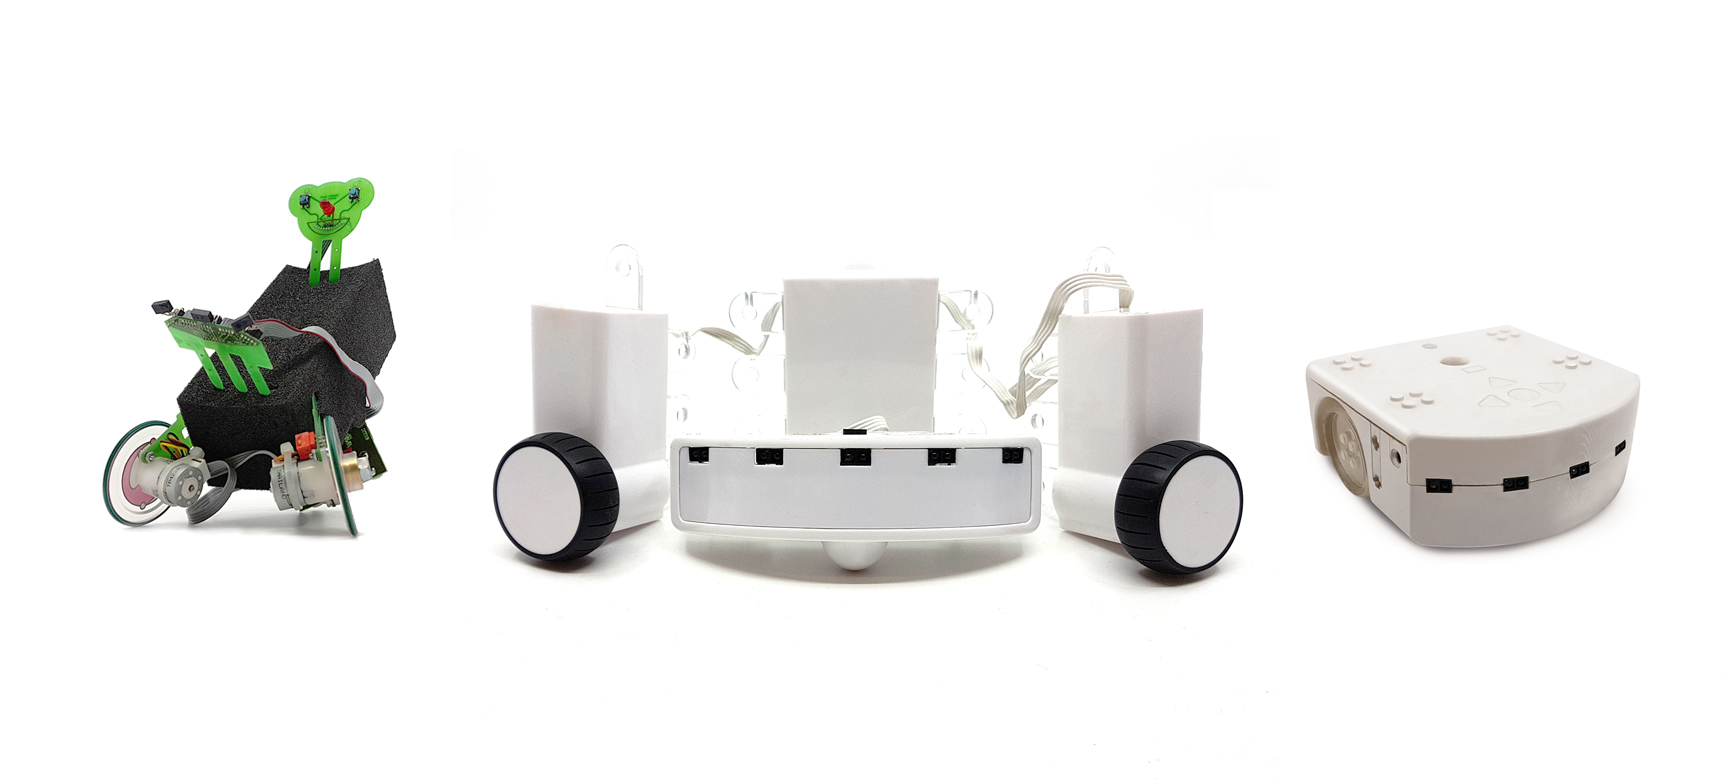
\includegraphics[width=\textwidth]{prototype_thymio_old}
  \caption{From left to right, "Monsieur Patate", Thymio, Thymio II}
  \label{fig:thymio_prototype}
\end{figure}

The result is a robot with a complex and complete set of sensors and actuators. 
The National Centre for Competence in Research (NCCR) Robotics research program supported the development of the robot whereas Mobsya, 
a non-profit organization that creates a robot, software, and educational activities to broaden young people's mind about technology and science, 
oversees the production, distribution, and communication of said robot. 
Every step of the Thymio project is open-source and has a non-profit aim to enhance the quality of it with the user's project and research, 
and reduce the cost and augment the lifetime for educational platforms and materials.

\begin{figure}
  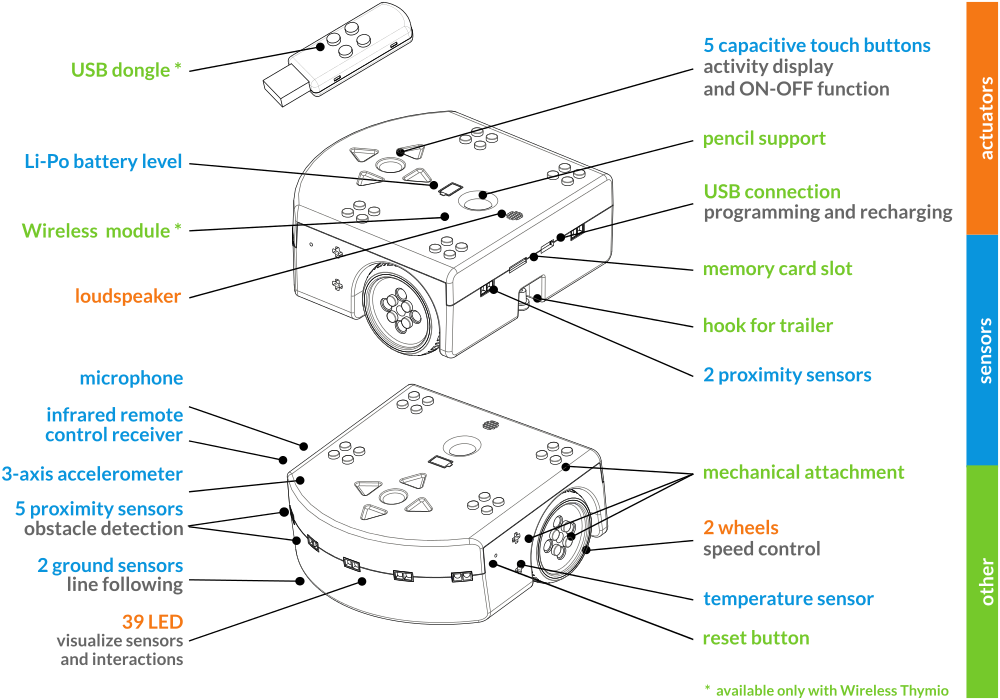
\includegraphics[width=\textwidth]{Wireless-thymioII-sensor-actuator-color-en}
  \caption{Thymio II sensor and actuator}
  \label{fig:thymio_sensor_actuator}
\end{figure}

\subsection{How does it works} \label{howdoesitworkref}

As seen in the figure above there exist two Thymio models, Thymio and Wireless Thymio. 
The difference between them lies in the ability of the second one to be programmed wirelessly, 
as its name suggests. To begin the creation of a program for the robot there exist two possibilities.
The first one, and the most common one for the public is done by using the software Aseba and a connected Thymio. 
In this case, the robot needs to be plugged in via USB cable or USB dongle (possible only if it is the Wireless Thymio) and powered on. 
Then the software can be used to connect to said robot and start to program in one of the four different programming languages, 
that are: VPL, Blockly, Aseba, and Scratch. Once the program is ready and sent to the robot it will be available to play. \\

The second option is to use the work-in-progress Thymio Suite version. 
This software doesn’t require a Thymio robot to be connected physically (or wirelessly) at all times as it has its own simulator built-in. 
The four said languages are still available, and one need to be chosen. 
After what comes the choice of connecting a physical Thymio or starting a simulation to emulate the programmed behaviour.

\subsection{The different programming languages}
\subsubsection{VPL}

One of the four different possibilities to program the Thymio is by using the visual programming language, or VPL, 
developed by the creator of Aseba. A visual programming language is an abstraction of the more common way to program. 
It is based on the manipulation of program elements graphically that can be manipulated following some spatial grammar to create a program. 
VPLs are based on a set of entities and relations, whereas most of the time entities are represented by boxes, 
or other graphical objects, and relations by simple arrows. They can be categorized into icon-based, 
form-based and diagram-based languages depending on the extent of visual expression inside of it. 
The use of visual programming languages can be found in multiple areas, such as the game engine “Unreal Engine 4” where their system of Blueprints is created upon a node-based VPL, 
or “Microsoft SQL Server Integration Services”. This abstraction allows easier access for neophytes, 
for example using graphic elements such as blocks, forms, diagrams, and others reduce drastically, if not eliminate, the syntactic errors made by the user.\\

In the case of the VPL developed by Aseba’s team, and the one we are mostly interested in, we have a programming language based on two types of blocks: Event blocks and Action blocks. 
From those two are built the seventeen, respectively eleven event blocks and six action blocks, entities. 
One of the main goals of VPL for Thymio was to let people who cannot yet read the ability to start programming and discover this world.\\

\begin{figure}
  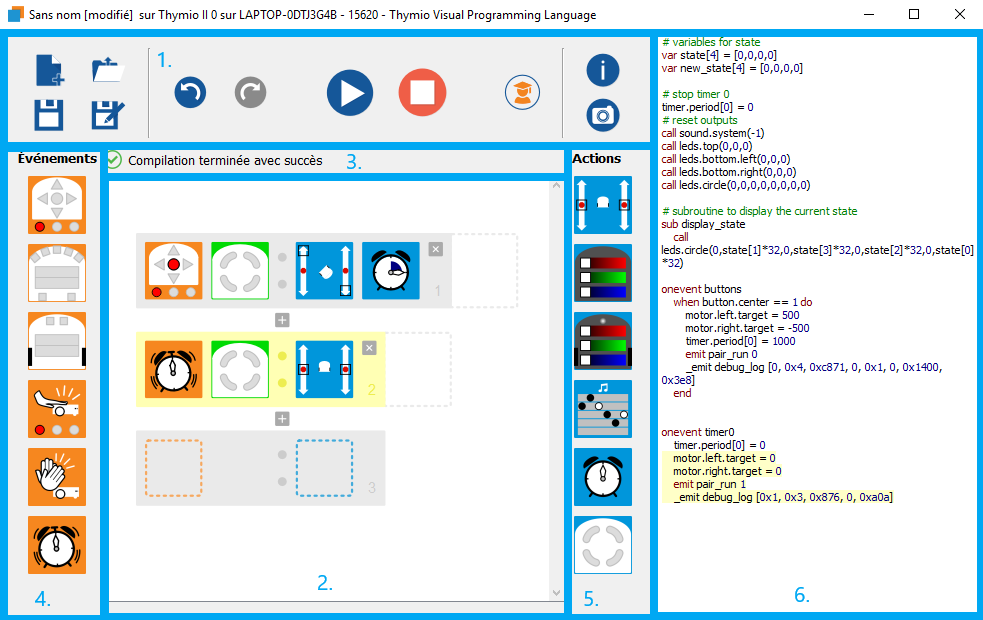
\includegraphics[width=\textwidth]{./VPL/Thymio_VPL_window}
  \caption{Thymio VPL Event and Action blocks}
  \label{fig:thymio_vpl_blocks}
\end{figure}

To begin creating a program follow the first steps described in the section \ref{howdoesitworkref} at the page \pageref{howdoesitworkref}. 
Once the VPL option has been chosen and the Thymio Visual Programming Language window appears we are ready to go. 
The window is split into six different regions with each of their purposes.
\begin{enumerate}
  \item A tool bar
  \item A programming window
  \item Console messages
  \item The event blocks
  \item The action blocks
  \item The program translated into AESL
\end{enumerate}

\begin{figure}
  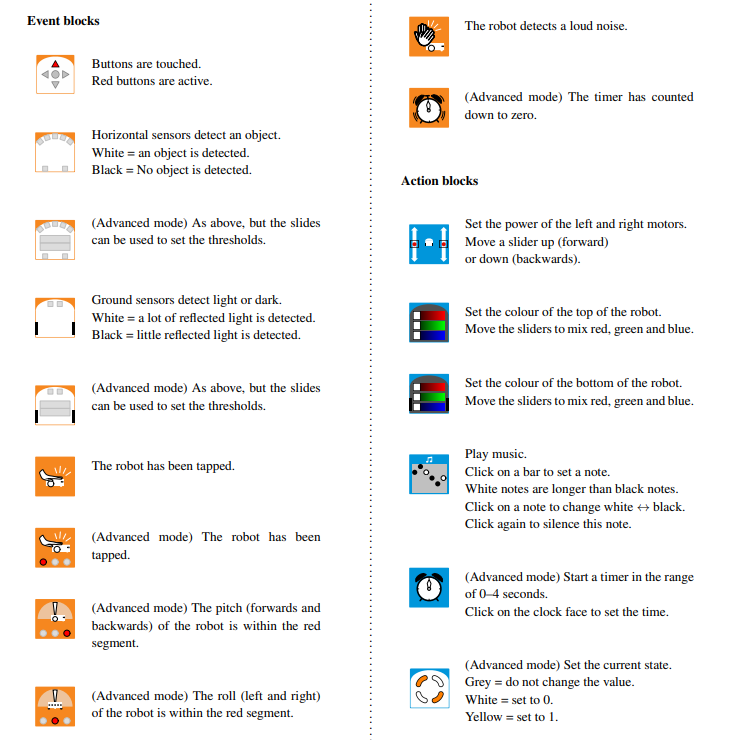
\includegraphics[width=\textwidth]{./VPL/Thymio_blocks}
  \caption{Thymio VPL Window}
  \label{fig:thymio_vpl_window}
\end{figure}

At first, the programming window will be empty of blocks, containing just a placeholder with empty slots. 
This placeholder is the base of every Thymio VPL program, it contains exactly one event block and one or more action block. 
This means that whenever the event of the event block happens then the set of actions added to this placeholder will occur at the same time. 
For example, with the following pair: \\
\begin{figure}
  \centering
  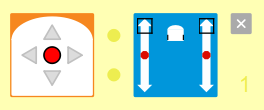
\includegraphics[scale=0.5]{./VPL/middlebtn_forward}
  \caption{Event and one Action relation}
  \label{fig:thymio_vpl_middlebtn_1e1a}
\end{figure}

Both wheels are powered to the maximum when the middle button is pressed. But more than one action can be attributed to one event, 
to do so simply drag another action block onto the previous pair, notice that the same block cannot be used twice for the same event. 
Here we turned the lights on top and set them to a complete green:\\
\begin{figure}
  \centering
  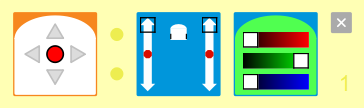
\includegraphics[scale=0.5]{./VPL/middlebtn_forward_green}
  \caption{Event and multiple Actions relation}
  \label{fig:thymio_vpl_middlebtn_1e2a}
\end{figure}

The maximum amount of action blocks we can add to an event is four, but we can add as many event blocks to our program as we want. 
Let us add two more event blocks to allow the robot to turn:\\
\begin{figure}
  \centering
  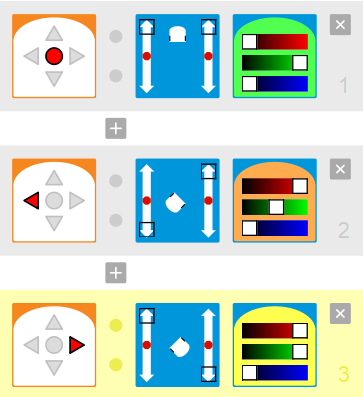
\includegraphics[scale=0.5]{./VPL/middlebtn_3E}
  \caption{Event and Actions relations}
  \label{fig:thymio_vpl_middlebtn_3e6a}
\end{figure}

Now we have a basic behavior, go straight with green lights when the middle button is pushed, turn left on itself with orange lights when the left button is pushed, 
and at last turn right on itself with yellow lights when the right button is pushed.\\

By clicking the button with a student as an icon we enable the advanced mode that gives us more possibilities for multiple blocks. It raises the amount of action block from four to six as well. \\

Let us refactor a bit the program from before, we will change the program by making the robot look left then right and starting over again using timers. 
To help us develop a more interesting program we have now access to a condition, a four led light on top of the robot, using this and the timer we can behave depending on the state of the robot. 
For example, hereafter the middle button was pressed a timer will start and after a short amount of time, it will light one particular led. 
Afterward, the event “timer elapsed” will be triggered but which pair should the program execute, turning right or turning left? 
Hence comes the use of the condition as we will execute the part of the program that corresponds to the state of the condition light. 
In this example, it will go back and forth between the two pairs: \\
\begin{figure}
  \centering
  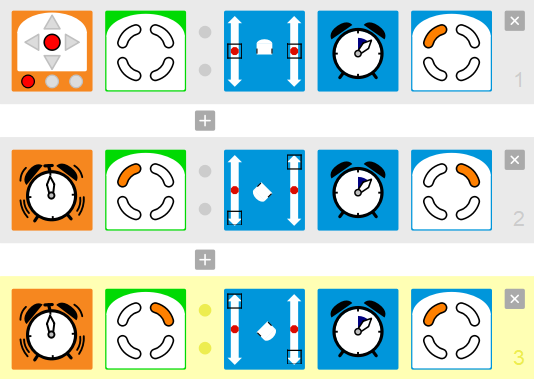
\includegraphics[scale=0.5]{./VPL/middlebtn_3E_adv}
  \caption{Advanced program}
  \label{fig:thymio_vpl_middlebtn_3e9a}
\end{figure}

\subsubsection{Blockly 4 Thymio}

The second possibility is to use Blockly4Thymio which is an environment based on Blockly. Blockly was released in May 2012 and was initially a replacement for OpenBlocks for the MIT App Inventor. 
It is an open-source client-side library that allows its users to easily add a block-based visual programming language to an application or website. 
Blockly is not in itself a programming language but rather used to create one. Its design makes it flexible and it can support a large set of features. 
As it is a visual programming language, we find the same advantages as the first possibility, such for example applying programming principles with no regard towards syntactic error.
Blockly is among the growing and most used visual programming environments because of a few important features. First, it can export the code generated with the blocks to one of the five following programming languages, 
as a built-in feature, JavaScript, Lua, Dart, Python, and PHP, and can be enhanced for any textual programming languages. 
The block pool can be expanded from its base pool or even reduced depending on the needs. The blocks are not restrained to only basic tasks and can implement sophisticated programming tasks. 
And it has been translated in over forty languages, and as well right-to-left versions. \\

Blockly includes a set of pre-defined blocks that can be used to develop with more ease the wanted application. They are arranged into eight families:
\begin{description}
  \item [Logic:] Blocks with Boolean definition, equality check, and conditions.
  \item [Loop:] Blocks for loops.
  \item [Math:] Blocks for numbers, arithmetic operation, a few basic math functions (for example cos, sin, square root) and some mathematical constant (Pi).
  \item [Text:] Blocks to create text and text operations.
  \item [Lists:] Blocks to create lists and standard list operation (length, get the value).
  \item [Color:] Blocks with a color definition.
  \item [Variables:] Blocks to create variables, and to set/get their values.
  \item [Functions:] Blocks to create functions, with return value or not, and to call existing function.
\end{description}

Each block holds a pre-assigned shape, thus restraining its usage to certain situations as a "hidden" way to control the syntax. Their shapes are defined by the different connections with other blocks, 
both external and internal, while external blocks describe what happens after or before, the internals describe what happens during or what are the arguments, logic. 
Following is a basic variable block with three external connectors, and a math block with the value of one, with one connector, that is assigned to the \texttt{Count} variable (the blocks need to be assembled). \\
\begin{figure}
  \centering
  
\includegraphics[scale=0.5]{./Blockly/basic_variable}
  \caption{Variable block}
  \label{fig:thymio_blockly_variable_block}
\end{figure}

Using the same logic as above we created a \texttt{Limit} variable with the value of 5 to demonstrate the next example. 
The block used is from the logic family and test whether the \texttt{Count} variable is smaller or equal to the \texttt{Limit} as internal blocks. 
It can then be added to a loop, a function or other statements that needs logic.\\
\begin{figure}
  \centering
  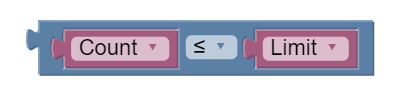
\includegraphics[scale=0.5]{./Blockly/basic_logic}
  \caption{Logic block}
  \label{fig:thymio_blockly_logic_block}
\end{figure}

Added to the base that Blockly is for Blockly4Thymio, is a compilator that interpret and adapt the Blockly code directly into Aseba language, and an Aseba Framework. 
Let us once again follow the steps described in the “How does it works” section in order to start blockly-ing a little program with Blockly4Thymio. 
Note that it is possible to open the Thymio Blockly environment without going through the Thymio suite, and without any Thymio II connected (physically or simulated). 
To do so open the location of Thymio, the downloaded not the installed, and select thymio\textunderscore blockly, and then index.
The environment window that opens after choosing the Blockly option is split into four parts.
\begin{enumerate}
  \item A tool bar
  \item A programming window
  \item The category of blocks
  \item The program translated into AESL
\end{enumerate}

\begin{figure}
  \centering
  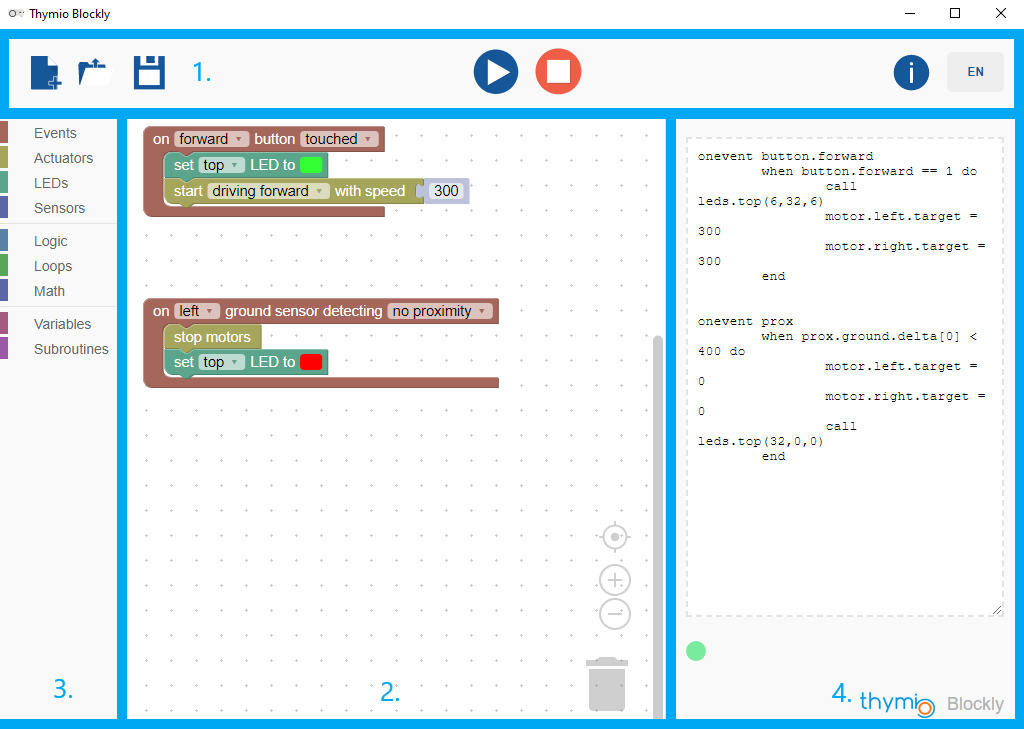
\includegraphics[scale=0.5]{./Blockly/blockly_window}
  \caption{Thymio Blockly window}
  \label{fig:thymio_blockly_window}
\end{figure}

The following figure demonstrates a simple program, once run the program listens to two different events. When the center button is pressed and when the front middle proximity sensor detects a wall. 
The first one will activate the two motors at the same speed, as to drive forward, and light the top LED to green. Whereas the second will stop the motors and turn the LED to red. \\
\begin{figure}
  \centering
  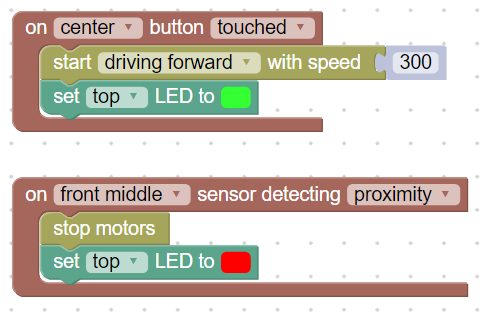
\includegraphics[scale=0.5]{./Blockly/forward_stop_wall}
  \caption{Basic program}
  \label{fig:thymio_blockly_basic_program}
\end{figure}

Here we set a variable to act as a control if Thymio is moving or not. We then use this information into a test when we click the middle button, and we either move forward or stop according to the result. 
We added two other events for the right and left buttons that are responsible to turn the robot.
\begin{figure}
  \centering
  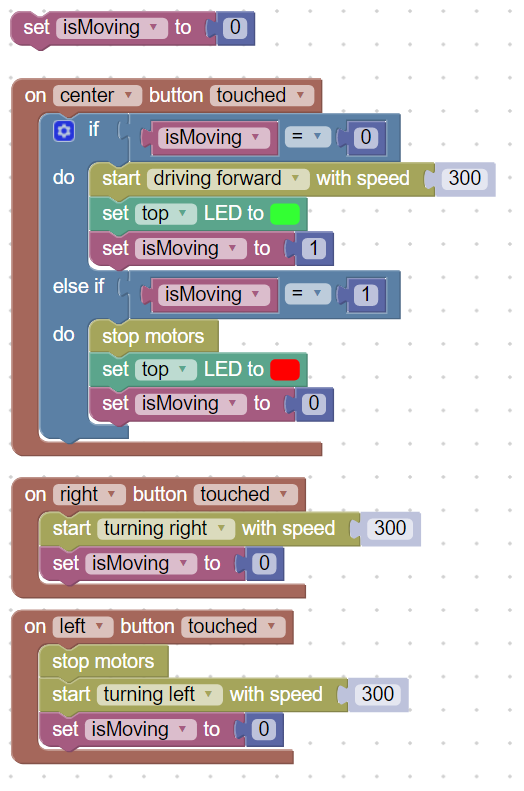
\includegraphics[scale=0.5]{./Blockly/advanced_program}
  \caption{More complex program}
  \label{fig:thymio_blockly_advanced_program}
\end{figure}

\subsubsection{Aseba}
\subsubsection{Scratch}
\subsection{What already exist} 
WeBots / Aseba logiciel
\section{Three JS}

\section{Requirements Documentation}
\subsection{Vision}
\subsection{Objectives}
\subsection{System Boundaries}
\subsection{Requirements}
\subsection{Risk Analysis}
Hack via .aesl as we execute the code if some code with malicious is feeded we still execute it.
What happens if part of the project aren't implemented ? How to bypass blockade? Security?
No financial risks.
\subsection{User Stories}
\textbf{\large Customer User Stories}

\subsection{Use Cases Model}
Use case diagram

\section{Architecture}
Domain class diagrams,
Domain model,
Package diagram,
Sequence diagram,
System sequence diagram

Write about the mvc, the interpreter pattern (?if used), problems because the three languages write files differently. All with the .aesl extension but not the same content format.


\section{Usefull latex commands (to be deleted later on)}
\lstset{language=JavaScript}
\begin{lstlisting}{basicstyle=\ttfamily\small}
  function generateBox(color, width, height, depth){

    var geometry = new THREE.BoxGeometry( width, height, depth );
    var material = new THREE.MeshPhongMaterial( { color : color} );
    var box = new THREE.Mesh( geometry, material );
                
    return box;
  }
\end{lstlisting}
For that we read the article book of \cite{Jerald:2015:VBH:2792790}
which is very interesting, much more than the article
\cite{Diniz:2017:UGO:3100317.3100324}

\section{Conclusion and future work}

\section{Appendices}
\subsection{Product Backlog}
\begin{longtable}{p{5mm}|p{2cm}|p{4cm}|p{1cm}|p{1cm}|p{1cm}|p{1cm}|p{1cm}}
  ID                     & Story Name & Story / Task Description & Priority & Est. Effort {[}h{]} & Update Effort {[}h{]} & Actual Effort{[}h{]} & Status                \\ \hline
  1 & Create Documentation & Develop and write the documentation & High & 108 & 52 &  & In-Progress \\ 
  2 & Set up the Environment & Setting up and configuring the development environment & High & 12 & 12 & 12 & Done \\ 
  3 & Basic Learning & Learning and training of the different technology used later on & High & 44 & 58 & 58 & Done \\ 
  4 & Develop Playgrounds & Create playgrounds and function to generate meshes & High & 40 & 48 & 48 & Done \\ 
  5 & Update Documentation & Update existing documentation & High &  &  &  & In-Progress \\
  6 & Architecture Implementation & Refactor the existing code into the designed architecture & High & 40 & 48 &  & In-Progress}\\ 
  7 & Web Deployement & Deploy the application on a webserver & High & 16 & 12 & 12 & Done \\ 
  8 & Basic UI & Implement a basic UI & Low & 8 & 4 &  & In-Progress \\ 
  9 & Behaviour Pipeline & Create pipeline to take .aesl file and translate/compile it into behaviour in javascript for the Thymio II & High &  &  &  & To Do \\ 
  10 & Phyisics Implementation & Implementation of Collisions for ThreeJS Meshes & High &  &  &  & To Do \\ 
  11 & Enhanced UI & Enhancement of the current UI & Low &  &  &  & To Do \\ 
  12 & Customizable Playgrounds & Implementation of a playground creator for users & High &  &  &  & To Do \\ 
  13 & Update Documentation & Update existing documentation and elaborate use cases and diagrams & High &  &  &  & To Do \\ 
  14 & Enhanced Behaviour Pipeline & Implement more sensors, action and event for Thymio II & High &  &  &  & To Do \\ 
  15 & Finish Documentation & Finish existing documentation & High &  &  &  & To Do \\
  16 & Prepare Defense & Prepare the defense & High &  &  &  & To Do \\ 
   &  &  & Total &  &  &  &  \\ 
\end{longtable}

\subsection{Sprint Backlog}
\subsubsection{First Sprint}
\textbf{2019-09-16 until 2019-10-07}
\begin{longtable}{p{5mm}|p{2cm}|p{4cm}|p{1cm}|p{1cm}|p{1cm}|p{1cm}|p{1cm}}
  ID                     & Story Name & Story / Task Description & Priority & Est. Effort {[}h{]} & Update Effort {[}h{]} & Actual Effort{[}h{]} & Status                \\ \hline
  1 & Create Documentation & Develop and write the documentation & High & 16 & 16 & 16 & Done \\ 
  1.1 & Template and Content & Choose a latex template and modify the content structure & High & 8 & 8 & 8 & Done \\ 
  1.2 & About Thymio & What is thymio and how does it work. & High & 8 & 8 & 8 & Done \\ 
  2 & Set up the Environment & Setting up and configuring the development environment & High & 12 & 12 & 12 & Done \\ 
  2.1 & GitHub & Create the project in GitHub and the Git environment & High & 4 & 4 & 4 & Done \\ 
  2.2 & Tools & Install Thymio Suite, NodeJS and download ThreeJS & High & 8 & 8 & 8 & Done \\ 
\end{longtable}

\subsubsection{Second Sprint}
\textbf{2019-10-07 until 2019-10-28}
\begin{longtable}{p{5mm}|p{2cm}|p{4cm}|p{1cm}|p{1cm}|p{1cm}|p{1cm}|p{1cm}}
  ID                     & Story Name & Story / Task Description & Priority & Est. Effort {[}h{]} & Update Effort {[}h{]} & Actual Effort{[}h{]} & Status                \\ \hline
  3 & Basic Learning & Learning and training of the different technology used later on & High & 44 & 58 & 58 & Done \\
  3.1 & ThreeJS & Read documentation and examples, and practice & High & 16 & 20 & 20 & Done \\ 
  3.2 & JavaScript & Update and deepen knowledge  & High & 8 & 8 & 8 & Done \\ 
  3.3 & Thymio languages & Learning and using VPL, Blockly, Aseba and Scratch & Medium & 24 & 30 & 30 & Done \\ 
  4 & Develop Playgrounds & Create playgrounds and function to generate meshes & High & 40 & 48 & 48 & Done \\ 
  4.1 & Two Default Playgrounds & Generating two defalut playground to be choosen for the simulator & Medium & 12 & 12 & 12 & Done \\ 
  4.2 & Thymio Model & Create or load Thymio model & Medium & 4 & 4 & 4 & Done \\ 
  4.3 & Mesh Generation & Create function to generate meshes for the playgrounds & High & 24 & 32 & 32 & Done \\ 
\end{longtable}

\subsubsection{Third Sprint}
\textbf{2019-10-28 until 2019-11-15}
\begin{longtable}{p{5mm}|p{2cm}|p{4cm}|p{1cm}|p{1cm}|p{1cm}|p{1cm}|p{1cm}}
  ID                     & Story Name & Story / Task Description & Priority & Est. Effort {[}h{]} & Update Effort {[}h{]} & Actual Effort{[}h{]} & Status                \\ \hline
  5 & Update Documentation & Update existing documentation & High &  &  &  & In-Progress \\
  5.1 & Four supported languages & Descibe and initiate to VPL, Blockly, Aseba and Scratch & High & 32 & 24 &  & In-Progress \\ 
  5.2 & Backlogs & Create the Sprint and Project backlog & High & 12 & 8 &  & In-Progress \\ 
  5.3 & Architecture & Create DCD, DM, PD, SD, SSD and proposition of architecture & High & 20 & 4 &  & In-Progress \\
  5.4 & User Stories & Formulate the User Stories & Medium & 8 &  &  & To Do \\ 
  5.5 & Risk Analysis & Create risk analysis & High & 12 &  &  & To Do \\ 
  6 & Architecture Implementation & Refactor the existing code into the designed architecture & High & 40 & 48 &  & In-Progress \\ 
  6.1 & Refactor Code & Refactor existing code into MVC Pattern & High & 20 & 44 & 44 & Done \\ 
  6.3 & Unit Testing & Write the JavaScript tests & High & 12 &  &  & To Do \\
  6.4 & JSDoc & Write the JavaScriptDoc & High & 8 & 4 &  & In-Progress \\ 
  7 & Web Deployement & Deploy the application on a webserver & High & 16 & 12 & 12 & Done \\ 
  7.1 & Virtual Machine Setup & Set up the Virtual machine & High & 8 & 4 & 4 & Done \\ 
  7.2 & WebServer & Create WebServer and publish it on bfh network & High & 8 & 8 & 8 & Done \\
  8 & Basic UI & Implement a basic UI & Low & 8 & 4 &  & In-Progress \\ 
  8.1 & Pages UI & Create three pages UI, one for each of the following index, simulation and creation pages & Low & 8 & 4 &  & In-Progress
\end{longtable}

\subsubsection{Fourth Sprint}
\textbf{2019-11-15 until 2019-12-09}
\begin{longtable}{p{5mm}|p{2cm}|p{4cm}|p{1cm}|p{1cm}|p{1cm}|p{1cm}|p{1cm}}
  ID                     & Story Name & Story / Task Description & Priority & Est. Effort {[}h{]} & Update Effort {[}h{]} & Actual Effort{[}h{]} & Status                \\ \hline
  9 & Behaviour Pipeline & Create pipeline to take .aesl file and translate/compile it into behaviour in javascript for the Thymio II & High &  &  &  & To Do \\ 
  10 & Phyisics Implementation & Implementation of Collisions for ThreeJS Meshes & High &  &  &  & To Do \\ 
\end{longtable}

\subsubsection{Fifth Sprint}
\textbf{2019-12-09 until 2019-12-30}
\begin{longtable}{p{5mm}|p{2cm}|p{4cm}|p{1cm}|p{1cm}|p{1cm}|p{1cm}|p{1cm}}
  ID                     & Story Name & Story / Task Description & Priority & Est. Effort {[}h{]} & Update Effort {[}h{]} & Actual Effort{[}h{]} & Status                \\ \hline
  11 & Enhanced UI & Enhancement of the current UI & Low &  &  &  & To Do \\ 
  12 & Customizable Playgrounds & Implementation of a playground creator for users & High &  &  &  & To Do \\ 
\end{longtable}

\subsubsection{Sixth Sprint}
\textbf{2019-12-30 until 2020-01-18}
\begin{longtable}{p{5mm}|p{2cm}|p{4cm}|p{1cm}|p{1cm}|p{1cm}|p{1cm}|p{1cm}}
  ID                     & Story Name & Story / Task Description & Priority & Est. Effort {[}h{]} & Update Effort {[}h{]} & Actual Effort{[}h{]} & Status                \\ \hline
  13 & Update Documentation & Update existing documentation and elaborate use cases and diagrams & High &  &  &  & To Do \\ 
  14 & Enhanced Behaviour Pipeline & Implement more sensors, action and event for Thymio II & High &  &  &  & To Do \\ 
  15 & Finish Documentation & Finish existing documentation & High &  &  &  & To Do \\
  15.1 & Create Video & Create the video file & High &  &  &  & To Do} \\ 
  15.2 & Prepare Presentation Day & Create the poster and the presentation for the Presentation Day & High &  &  &  & To Do} \\
  15.3 & Write in the Book & Write the page for the Book & High & 8 & 4 &  & To Do} \\ 
  15.4 & Finish Writting Documentation & Terminate the writting part of the documentation & High &  &  &  & To Do} \\ 
  15.5 & Prepare to Submit & Check spelling mistake, check images, print it, put the project on a USB stick & High &  &  &  & To Do} \\ \hline
\end{longtable}

\subsubsection{Seventh Sprint}
\textbf{2020-01-18 until 2020-01-end}
\begin{longtable}{p{5mm}|p{2cm}|p{4cm}|p{1cm}|p{1cm}|p{1cm}|p{1cm}|p{1cm}}
  ID                     & Story Name & Story / Task Description & Priority & Est. Effort {[}h{]} & Update Effort {[}h{]} & Actual Effort{[}h{]} & Status                \\ \hline
  16 & Prepare Defense & Prepare the defense & High &  &  &  & To Do \\ 
\end{longtable}

\subsection{Gantt Diagram}
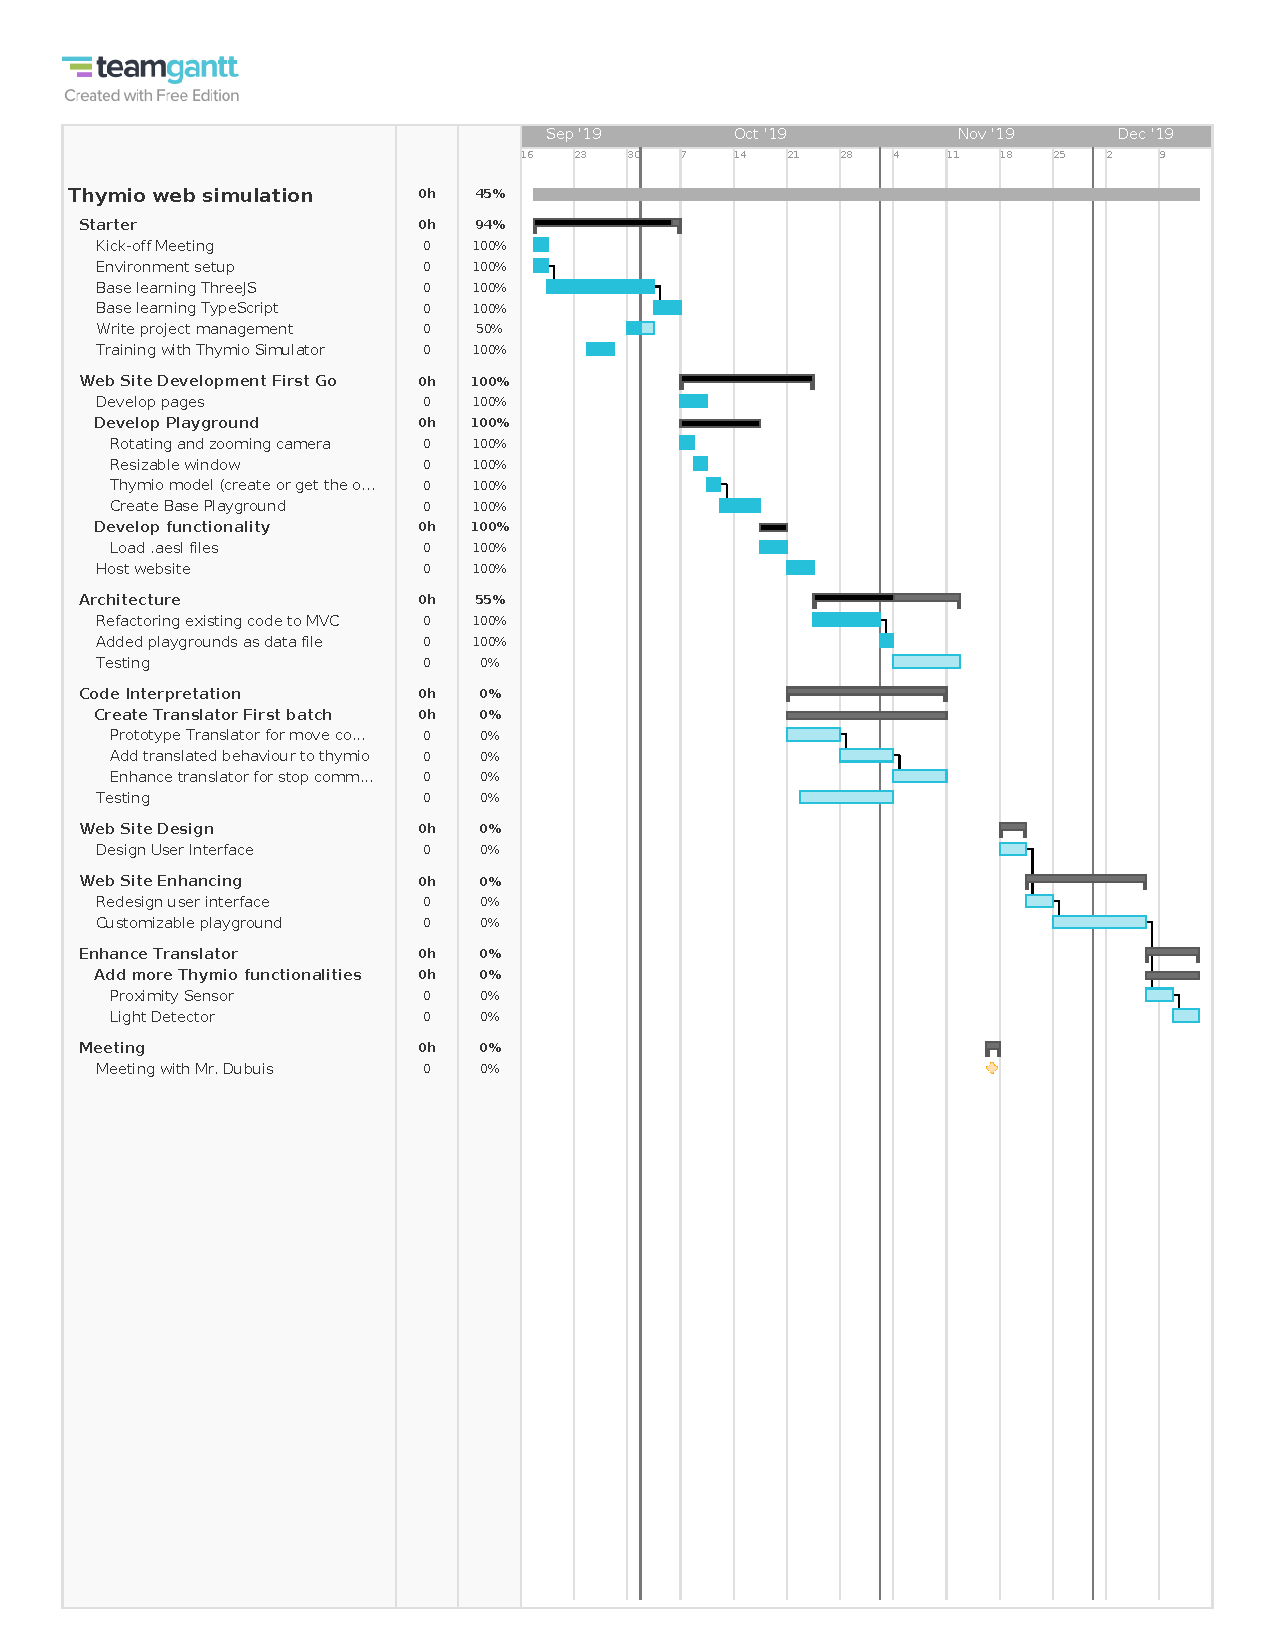
\includepdf[pages=-, pagecommand={}, width=\textwidth]{Thymio_web_simulation_Gantt.pdf}

\subsection{Version control}

\subsection{Configuration}

\textbf{User information} \\
On demand.\\

\textbf{Access the Windows Virtual Machine}\\
\begin{center}
  \begin{tabular}{|c|c|c|}
    \hline
     & Linux WM -ssh & Windows VM - rdp \\
    \hline
    Windows & Putty & Remote Desktop Connection \\
    \hline
    Linux & terminal & Remmina \\
    \hline
    MacOS & terminal & Microsoft Remote Desktop \\
    \hline
  \end{tabular}
\end{center}\\

See link bellow for more information and links. (It requires to be inside the bfh networkd to access it)
\url{https://intranet.bfh.ch/TI/fr/Studium/Bachelor/Informatik/Tools/VMsHowto/Pages/default.aspx?k=vm}\\

\textbf{First Configuration of IIS manager}\\

We followed the steps in this tutorial video in order to configure IIS. \url{https://www.youtube.com/watch?v=rPRLe7QeVHM}

Then we had to open the port in order to access it from within the LAN.
\begin{enumerate}
  \item Open the windows Firewall, click on Inbound Rules and New Rule. This will open the New Inbound Rule Wizard.
  \item Select the desired type, Port, click next.
  \item Choose TCP and specify the port used, here 80, click next.
  \item Select Allow connection, click next.
  \item Select all three profile options, click next.
  \item Add a Name and a description to this rule, click finish.
\end{enumerate}

With this specified the website is now accessible from within the LAN at the following adress : http://147.87.116.44/Code/HTML \\

\textbf{Additional setup}\\

It was needed to create a web.config file and add a few file extension so that the .mtl and .obj would still be able to load. 
Otherwise we encountered an error of the type "Failed to load resource: the server responded with a status of 404 (Not Found)." 
The text that needed to be added to the web.config file is the following : \\
\lstset{language=XML}
\begin{lstlisting}{basicstyle=\ttfamily\small}
<?xml version="1.0" encoding="UTF-8"?>
  <configuration>
    <system.webServer>
         <staticContent>
           <remove fileExtension=".mtl" />
           <mimeMap fileExtension=".mtl" mimeType="text/plain" />
           <mimeMap fileExtension=".obj" mimeType="application/octet-stream" />
         </staticContent>
    </system.webServer>
</configuration>
\end{lstlisting}

\subsection{Meetings}
\begin{tabular}{ | m{3cm} | m{10cm} | }
  \hline
  Date & Content \\
  \hline
  17.09.2019 & \textbf{Kick Off meeting}\\
  & - Documentation/Management\\
  & - Technology to use : ThreeJS and Typescript\\
  & - Setting up the goals\\
  \hline
  24.09.2019 & \textbf{Second meeting} \\
  & - Documentation language : English \\
  & - Thymio model \\
  & - Base talk about riks management \\
  \hline
  08.10.2019 & \textbf{Third meeting}\\
  & Workplace\\
  & - Discussion on the choice of Windows as the Virtual Machine \\
  & - Create a configuration file with the information of the VM \\
  & - And an architecture proposal \\
  \hline
  15.10.2019 & \textbf{Fourth meeting} \\
  & - Which shapes and meshes should the user be able to create for his own custom playground \\
  & - Problems with webserver, has to be accessible from outside the vm, so maybe switching from windosw to linux \\
  & - Talk about the problem of thymio suite, that is the software allows the user to create programs only if a physical or a simulated one is plugged in \\
  \hline
  25.10.2019 & \textbf{Fifth meeting} \\
  & - Discussed using a Finite state machine to handle the events, but it may be too rigid so a non-deterministic finite state machine was the possible solution we came with \\
  & - First little talk about the meeting with the expert, report\\
  \hline
\end{tabular}

\listoffigures

\section{Problems encountered}
\begin{itemize}
  \item javascript not refreshing properly due to cache -> disable cache
  \item 3d Model not loaded on the webserver -> first tried to change the directory, then mixed two solution. 
        Had to create a web.config file and add file extension for .mtl and .obj.
        https://stackoverflow.com/questions/41245938/web-server-cannot-find-mtl-file
        https://stackoverflow.com/questions/16097580/three-js-loading-obj-error-in-azure-but-not-locally
  \item shadow not rendering on plane of all playgrounds
  \item javascript file not found on server, net::ERR\textunderscore ABORTED 404 (Not Found) => first solution (working partially) was to add a IIS\textunderscore IUSRS.
  \item Thymio Blockly has trouble loading saved files. Using the software I wasn't able to load any .aesl file previously created with it, but I could load them if I used the index.html one.
\end{itemize}

%% Print the bibibliography and add the section to the table of content
\printbibliography[heading=bibintoc]

\end{document}
